\documentclass[12pt]{article}
\usepackage[a4paper, top=0.8in, bottom=0.7in, left=0.8in, right=0.8in]{geometry}
\usepackage{amsmath}
\usepackage{amsfonts}
\usepackage{graphicx}
\usepackage{fancyhdr}
\usepackage{tcolorbox}
\usepackage{enumitem}
\usepackage{setspace}
\usepackage{pgfplots}
\usepackage[defaultfam,tabular,lining]{montserrat} % Font settings for Montserrat

\setlength{\parindent}{0pt}
\pagestyle{fancy}

\setlength{\headheight}{27.11148pt}
\addtolength{\topmargin}{-15.11148pt}

\fancyhf{}
%\fancyhead[L]{\textbf{6.NS.C.6, 6.NS.C.7: Number Lines and Inequalities - Answer Key}}
\fancyhead[R]{
\includegraphics[width=0.8cm]{Round Logo.png}}
\fancyfoot[C]{\footnotesize © Study Smart Tutors}

\sloppy

\pgfplotsset{compat=1.18}

\begin{document}

\subsection*{Problem Set: Number Lines and Inequalities - Answer Key}
\onehalfspacing

% Learning Objective Box
\begin{tcolorbox}[colframe=black!40, colback=gray!5, 
coltitle=black, colbacktitle=black!20, fonttitle=\bfseries\Large, 
title=Learning Objective, halign title=center, left=5pt, right=5pt, top=5pt, bottom=5pt]
\textbf{Objective:} \small Develop an understanding of how to locate numbers on a number line, compare rational numbers, and interpret inequalities in real-world contexts.
\end{tcolorbox}

% Exercises Box
\begin{tcolorbox}[colframe=black!60, colback=white, 
coltitle=black, colbacktitle=black!15, fonttitle=\bfseries\Large, 
title=Exercises, halign title=center, left=10pt, right=10pt, top=10pt, bottom=20pt]
\begin{enumerate}[itemsep=1.5em]
    \item Plot the following numbers on a number line: \( -3, 2.5, 0, -1.5, 4 \).\\
    \textcolor{red}{\textbf{Solution:} Plot \( -3, -1.5, 0, 2.5, 4 \) on the number line. Numbers to the left are smaller.}
    \begin{center}
        \begin{tikzpicture}
            \draw[thick, <->] (-5.5,0) -- (5.5,0);
            \foreach \x in {-5,-4,-3,-2,-1,0,1,2,3,4,5} {
                \draw (\x,0.1) -- (\x,-0.1) node[below] {\x};
            }
            \foreach \x in {-3,-1.5,0,2.5,4} {
                \filldraw (\x,0) circle (2pt);
            }
        \end{tikzpicture}
    \end{center}
    
    \item Compare the numbers \( -7 \) and \( -4 \). Write the inequality and explain which is greater.\\
    \textcolor{red}{\textbf{Solution:} \( -4 > -7 \) because \( -4 \) is closer to \( 0 \) on the number line.}

    \item Order the numbers \( 1.2, -0.8, 0, -1.5, 2.5 \) from least to greatest.\\
    \textcolor{red}{\textbf{Solution:} Order: \( -1.5, -0.8, 0, 1.2, 2.5 \).}

    \item Solve and graph: \( x + 3 \leq 5 \).\\
    \textcolor{red}{\textbf{Solution:} Subtract \( 3 \): \( x \leq 2 \).}
    \vspace{1em}
    \begin{center}
        \begin{tikzpicture}
            \draw[thick, <->] (-3,0) -- (6,0);
            \foreach \x in {-2,-1,0,1,2,3,4,5} {
                \draw (\x,0.1) -- (\x,-0.1) node[below] {\x};
            }
            \draw[fill=black] (2,0) circle (2pt);
            \draw[thick] (2,0) -- (-3,0) [dashed];
        \end{tikzpicture}
    \end{center}
    
    \item Write the inequality: "The temperature is less than or equal to \( -5^\circ \)C."\\
    \textcolor{red}{\textbf{Solution:} \( x \leq -5^\circ \).}

    \item Compare and write the inequality: \( 2.4 \) and \( 2.5 \).\\
    \textcolor{red}{\textbf{Solution:} \( 2.4 < 2.5 \).}

    \item Plot and label \( -\frac{5}{6}, \frac{2}{3}, \frac{1}{2} \) on a number line.\\
    \textcolor{red}{\textbf{Solution:} Plot each fraction at its correct position between \( -1 \) and \( 1 \).}
    \begin{center}
        \begin{tikzpicture}
            \draw[thick, <->] (-1.5,0) -- (1.5,0);
            \foreach \x in {-1,0,1} {
                \draw (\x,0.1) -- (\x,-0.1) node[below] {\x};
            }
            \filldraw (-0.83,0) circle (2pt) node[above] {\(-\frac{5}{6}\)};
            \filldraw (0.67,0) circle (2pt) node[above] {\(\frac{2}{3}\)};
            \filldraw (0.5,0) circle (2pt) node[above] {\(\frac{1}{2}\)};
        \end{tikzpicture}
    \end{center}

    \item Solve for \( y \): \( -4 \leq y + 2 < 3 \). Graph the solution.\\
    \textcolor{red}{\textbf{Solution:} Subtract \( 2 \): \( -6 \leq y < 1 \).}
    \vspace{1em}
    \begin{center}
        \begin{tikzpicture}
            \draw[thick, <->] (-7,0) -- (2,0);
            \foreach \x in {-6,-5,-4,-3,-2,-1,0,1} {
                \draw (\x,0.1) -- (\x,-0.1) node[below] {\x};
            }
            \draw[fill=black] (-6,0) circle (2pt);
            \draw[fill=white] (1,0) circle (2pt);
            \draw[thick] (-6,0) -- (0.99,0);
        \end{tikzpicture}
    \end{center}
\end{enumerate}
\end{tcolorbox}

% Problems and Performance Task will include the same structure.

% Problems Box (Part 1)
\begin{tcolorbox}[colframe=black!60, colback=white, 
coltitle=black, colbacktitle=black!15, fonttitle=\bfseries\Large, 
title=Problems (Part 1), halign title=center, left=10pt, right=10pt, top=10pt, bottom=40pt]
\textbf{Solve the following problems. Show all work.}

\begin{enumerate}[start=9, itemsep=5em]

    % Problem 9
   \item A submarine is at \( -200 \) feet. It ascends \( 120 \) feet. Where is the submarine now on a number line?

    \begin{tikzpicture}[scale=1.5]
        % Vertical number line
        \draw[thick, <->] (0,-2.5) -- (0,2); 
        
        % Tick marks and labels
        \foreach \y in {-2,-1,0,1} {
            \draw (-0.1,\y) -- (0.1,\y) node[right] {{\y00}};
        }
    \end{tikzpicture}

    {\color{red} Solution: Starting depth is \( -200 \). After ascending \( 120 \), calculate:
    \[
    -200 + 120 = -80.
    \]
    The submarine is now at **\(-80\) feet**.}

    % Problem 10
    \item The freezing point of a substance is \( -15^\circ \text{C} \), and its boiling point is \( 85^\circ \text{C} \). What is the range of temperatures where the substance is in a liquid state? Write an inequality to represent this.

    {\color{red} Solution: A substance is liquid between freezing and boiling:
    \[
    -15 < T < 85.
    \]
    The temperature range is **\(-15^\circ C\) to \( 85^\circ C\)**.}
    
\end{enumerate}
\end{tcolorbox}

\vspace{1em}

% Problems Box (Part 2)
\begin{tcolorbox}[colframe=black!60, colback=white, 
coltitle=black, colbacktitle=black!15, fonttitle=\bfseries\Large, 
title=Problems (Part 2), halign title=center, left=10pt, right=10pt, top=10pt, bottom=40pt]
\begin{enumerate}[start=11, itemsep=5em]

    % Problem 11
    \item A delivery truck’s load weight must be greater than \( 500 \) pounds and less than or equal to \( 1,000 \) pounds.  
    \begin{enumerate}
        \item Write an inequality to represent the allowable range of the load weight.  
            {\color{red} Solution: Let \( w \) be the truck’s weight:
            \[
            500 < w \leq 1,000.
            \]}
        
        \item If the truck currently carries \( 620 \) pounds, is the load within the acceptable range? If so, how many more pounds can the truck carry?
        
            {\color{red} Solution: Since \( 500 < 620 \leq 1,000 \), the load is within range.  
            Maximum additional weight:
            \[
            1,000 - 620 = 380.
            \]
            The truck can carry **up to 380 more pounds**.}
    \end{enumerate}

    % Problem 12
    \item Compare and explain: Which is greater, \( -2.7 \) or \( -2.9 \)? Write your answer as an inequality and explain.

    {\color{red} Solution: **Numbers further right on the number line are greater.**  
    Since \( -2.7 \) is to the right of \( -2.9 \), we write:
    \[
    -2.7 > -2.9.
    \]
    **Explanation:** A less negative number is always greater than a more negative number.}
    
    {\color{blue} Instructor Note: If students struggle, ask them to compare money: Is losing **\$2.70** better than losing **\$2.90**?}
    
\end{enumerate}
\end{tcolorbox}



% Performance Task Box (Part 1)
\begin{tcolorbox}[colframe=black!60, colback=white, 
coltitle=black, colbacktitle=black!15, fonttitle=\bfseries\Large, 
title=Performance Task: Mountain Heights and Depths (Part 1), halign title=center, left=10pt, right=10pt, top=10pt, bottom=60pt]
\textbf{Scenario:} A mountain peak is at \( 14,000 \) feet above sea level, and a nearby valley is \( -200 \) feet below sea level. A helicopter starts at the peak and descends to the valley.

\textbf{Task:}
\begin{enumerate}[itemsep=5em]

    \item Write the inequality representing the helicopter's altitude during the descent.
    
        {\color{red} Solution: Since the helicopter starts at 14,000 feet and descends to -200 feet, the altitude \( h \) is:
        \[
        -200 \leq h \leq 14,000.
        \]}

    \item Graph the altitude on a number line.

    \begin{center}
    \begin{tikzpicture}
        % Draw number line
        \draw[thick, <->] (-2,0) -- (6,0);
        % Tick marks
        \foreach \x in {-1,0,1,2,3,4,5} {
            \draw (\x,0.1) -- (\x,-0.1);
        }
        % Labels
        \node at (-1, -0.4) {\(-200\)};
        \node at (5, -0.4) {\(14,000\)};
        % Line segment to represent altitude range
        \draw[thick, blue] (-1,0) -- (5,0);
    \end{tikzpicture}
    \end{center}

    {\color{red} Solution: The number line represents the range **from -200 feet to 14,000 feet**.}
    
\end{enumerate}
\end{tcolorbox}

\vspace{1em}

% Performance Task Box (Part 2)
\begin{tcolorbox}[colframe=black!60, colback=white, 
coltitle=black, colbacktitle=black!15, fonttitle=\bfseries\Large, 
title=Performance Task: Mountain Heights and Depths (Part 2), halign title=center, left=10pt, right=10pt, top=10pt, bottom=60pt]
\begin{enumerate}[start=3, itemsep=5em]

    \item If the helicopter stops halfway between the peak and the valley, what is its altitude? Show your work.
    
        {\color{red} Solution: Halfway point formula:
        \[
        \frac{\text{Max} + \text{Min}}{2} = \frac{14,000 + (-200)}{2}.
        \]
        Simplify:
        \[
        \frac{14,000 - 200}{2} = \frac{13,800}{2} = 6,900.
        \]
        The helicopter stops at **6,900 feet**.}
        
        {\color{blue} Instructor Note: Remind students to check their work by finding the difference between **6,900** and both **14,000** and **-200**—it should be equal.}
\end{enumerate}
\end{tcolorbox}











% Reflection Box
\begin{tcolorbox}[colframe=black!60, colback=white, 
coltitle=black, colbacktitle=black!15, fonttitle=\bfseries\Large, 
title=Reflection, halign title=center, left=10pt, right=10pt, top=10pt, bottom=110pt]
What strategies did you use to locate numbers on a number line and solve inequalities? Reflect on any challenges you encountered and how you overcame them.
\end{tcolorbox}

\end{document}
